\section{Experimentación y resultados}
\label{sec:resultados}

\subsection{La serie final}

La serie final comprende veintiséis candidatos, de los cuales veinticinco se
evaluaron en el leaderboard público; P123 quedó listo pero no se envió. En
total, el proyecto realizó 47 envíos de modelos al leaderboard (más una
sonda de plantilla); 25 corresponden a esta
serie. La Tabla~\ref{tab:serie} reúne todos los experimentos con su métrica local en
las dos particiones congeladas, su $F_1$ público y la decisión registrada.
Las cifras locales se re-ejecutaron desde las probabilidades OOF; las del
leaderboard son el registro externo de Kaggle y no son recomputables.

\begin{table*}[t]
\centering
\caption{La serie final (P108--P133, sin P123). CCV es la $F_1$ media
columnar out-of-fold sobre las 1\,483 filas de desarrollo; LB es el $F_1$
público de Kaggle. P123 no se envió y se omite. El registro interno del
leaderboard guarda la media de las dos particiones; aquí se reportan por
separado.}
\label{tab:serie}
\scriptsize
\setlength{\tabcolsep}{4.5pt}
\begin{tabular*}{\textwidth}{@{\extracolsep{\fill}}lrrrl@{}}
\toprule
Exp. & CCV canónica & CCV partición 47 & LB público & Decisión \\
\midrule
P108 & 0.782372 & 0.781185 & 0.78855 & Adoptado \\
P109 & 0.792215 & 0.789294 & 0.77447 & Descartado (min\_df=5) \\
P110 & 0.784998 & 0.784318 & 0.78967 & Mejor LB \\
P111 & 0.786912 & 0.785868 & 0.78951 & Descartado \\
P112 & 0.780834 & 0.781824 & 0.78652 & Descartado \\
P113 & 0.787241 & 0.785049 & 0.78664 & Descartado \\
P114 & 0.787218 & 0.785673 & 0.79057 & Mejor LB \\
P115 & 0.788431 & 0.787190 & 0.78825 & Descartado \\
P116 & 0.786348 & 0.788892 & 0.78975 & Descartado \\
P117 & 0.787967 & 0.787259 & 0.78885 & Descartado \\
P118 & 0.787881 & 0.786026 & 0.78930 & Descartado \\
P119 & 0.785897 & 0.784121 & 0.78860 & Descartado \\
P120 & 0.787582 & 0.785673 & 0.79035 & Descartado \\
P121 & 0.787582 & 0.785673 & 0.79095 & Mejor LB \\
P122 & 0.787582 & 0.786034 & 0.79095 & Empate técnico \\
P124 & 0.787127 & 0.785810 & 0.79095 & Neutral \\
P125 & 0.787127 & 0.785810 & 0.79337 & Mejor LB \\
P126 & 0.787127 & 0.785810 & 0.79375 & Mejor LB \\
P127 & 0.787582 & 0.786034 & 0.79517 & Mejor LB \\
P128 & 0.787582 & 0.786034 & 0.80516 & Mejor LB histórico \\
P129 & 0.787582 & 0.786034 & 0.80078 & Descartado (offset 4.0) \\
P130 & 0.787582 & 0.786034 & 0.80516 & Empate técnico \\
P131 & 0.787582 & 0.786034 & 0.80872 & Mejor LB \\
P132 & 0.787582 & 0.786034 & 0.81279 & Mejor LB ($>0.81$) \\
P133 & 0.787582 & 0.786034 & 0.81447 & Envío final \\
\midrule
\multicolumn{5}{l}{\scriptsize * P123 (CCV 0.788584 / 0.786034) quedó listo en desarrollo local y no se envió a Kaggle.} \\
\bottomrule
\end{tabular*}
\end{table*}

\subsection{Qué funcionó}

La primera ganancia vino de la representación. P108 sustituyó la unión de dos
bloques de V03 por V2\_triple y pasó de 0.777211 a 0.782372 en la partición
canónica ($+0.005160$) y de 0.78306 a 0.78855 en el leaderboard
($+0.00549$). La mejora se replicó en la partición 47 ($+0.005553$), de modo
que no fue una fluctuación de una sola partición.

La segunda ganancia vino del ensamble. P110 mezcló 95\,\% de la regresión
logística con 5\,\% de SGD y subió a 0.784998 local y 0.78967 en el
leaderboard. P114 añadió SAGA con ElasticNet, calibró la temperatura en 1.04
y alcanzó 0.787218 local ($+0.002220$ sobre P110) y 0.79057 en el
leaderboard. La mejora se observó en cuatro de los cinco pliegues de la
partición canónica y en tres de los cinco de la partición 47. El
Tri-Optimizer se convirtió en la base de todo lo que siguió: a partir de
P114 el proyecto dejó de cambiar la representación y los modelos, y concentró
el esfuerzo en la decisión.

La tercera ganancia vino de las leyes de decisión. P121 fijó el staging
asimétrico y el ancla de prevalencia: 0.79095 en el leaderboard. El salto
grande llegó con los pares compensados. P125 sumó el primer par doble
($+0.00242$), P126 el segundo ($+0.00038$), P127 el tercero ($+0.00142$) y
P128 el lote de quince pares que cruzó la barrera de 0.80
($+0.00999$). Después de P128, P131 recuperó la fila 114 y sumó siete pares
($+0.00356$, primer lugar), P132 sumó otros siete ($+0.00407$, primer
registro por encima de 0.81) y P133 sumó nueve ($+0.00168$, 0.81447). La
Figura~\ref{fig:escalera} muestra la divergencia entre la métrica local y el
leaderboard: las variantes P127--P133 comparten exactamente la misma CCV
porque sus reglas no disparan en entrenamiento; P124--P126, con la escalera
histórica, quedan en 0.787127. Solo el leaderboard las distingue.

\begin{figure*}[t]
\centering
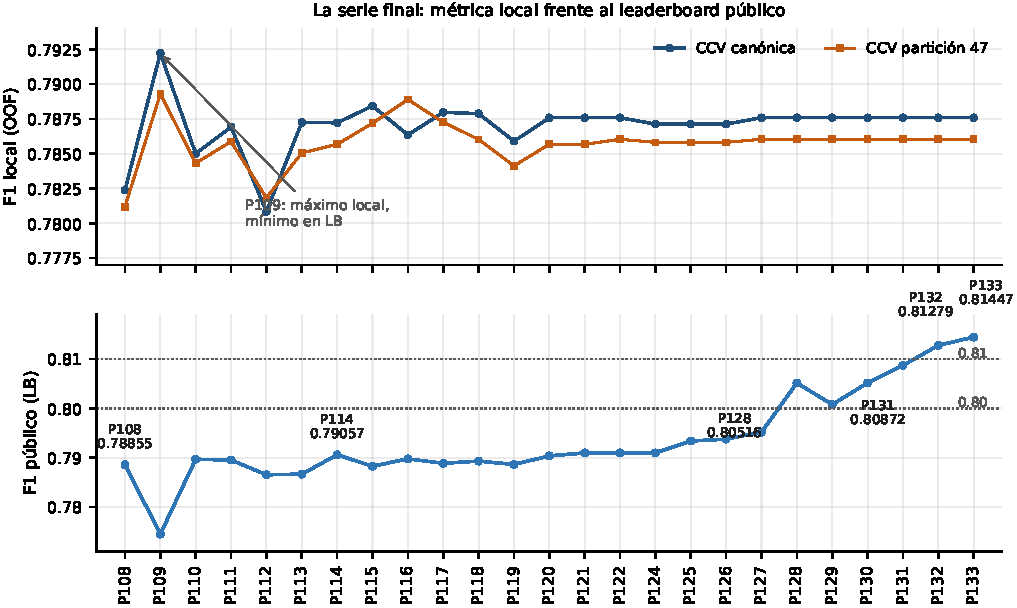
\includegraphics[width=\textwidth]{fig_escalera.pdf}
\caption{La serie final. Arriba: $F_1$ out-of-fold en las dos particiones
congeladas. Abajo: $F_1$ público de Kaggle. P109 es el caso paradigmático de
divergencia: la mejor métrica local de la serie (0.792215) produjo el peor
resultado público (0.77447). Las variantes P127--P133 comparten la misma
métrica local porque sus reglas léxicas no aparecen en entrenamiento;
P124--P126 usan la escalera histórica y quedan en 0.787127.}
\label{fig:escalera}
\end{figure*}

\subsection{Qué no funcionó}

El fracaso más instructivo fue P109. La poda por frecuencia
(\texttt{min\_df}=5) y la recalibración de umbrales produjeron la mejor
métrica local de toda la serie (0.792215 canónica, 0.789294 en la partición
47), pero el leaderboard cayó a 0.77447, por debajo de V03. La explicación es
mecánica: la poda elimina términos raros que sostienen la señal en un corpus
pequeño; la validación local, al compartir el mismo vocabulario podado,
sobreestima la transferencia. P109 se rechazó y se convirtió en la evidencia
de que la decisión debía mirar el leaderboard, no solo la CCV.

La familia de ensambles alternativos tampoco superó a P114. P111 (mezcla
95/5 con $C$ adaptada) quedó en 0.78951; P112 (bagging de diez pliegues) en
0.78652; P113 (tri-blend con pérdida de margen) en 0.78664. P115 (gating
ontológico dual) mejoró la métrica local hasta 0.788431 pero cayó a 0.78825
en el leaderboard: los rescates sobrepredijeron positivos en el test ciego.
P116--P119 exploraron \texttt{max\_df}=0.90, NBSVM, BM25 con SVD y un canal
de mención; ninguno superó a P114 en el leaderboard (0.78975, 0.78885,
0.78930 y 0.78860). P120, con las tres leyes de staging completas, quedó en
0.79035; P122 y P124 empataron con P121 en 0.79095.

P129 es el contraejemplo de la Proposición~\ref{prop:par}. Once pares con un
desplazamiento forzado de $+4.0$ en log-odds saturaron la probabilidad
($\sigma(z+4)>0.98$), rompieron la escala del ranking e hicieron perder tres
predicciones positivas de TR que el envío anterior conservaba. El resultado fue
0.80078, una
caída de 0.00438 frente a P128. P130 intentó suprimir la fila 114 (una cita
irónica de \emph{Dr. House}) y empató exactamente con P128 en 0.80516: la
supresión anuló el beneficio de los rescates. La lección fue doble: las
frases de ficción no se suprimen sin evidencia inequívoca y los lotes deben
ser pequeños, contables y con desplazamientos moderados. La
Tabla~\ref{tab:rechazos} detalla, para cada candidato descartado, la
hipótesis que lo motivó y la razón concreta del rechazo.

\begin{table*}[t]
\centering
\caption{Por qué se rechazaron los candidatos de la serie final que no
llegaron a campeones. La primera cifra de cada resultado es la CCV canónica y
la segunda el LB público.}
\label{tab:rechazos}
\scriptsize
\begin{tabularx}{\textwidth}{@{}>{\raggedright\arraybackslash}p{1.5cm}>{\raggedright\arraybackslash}p{4.3cm}>{\raggedright\arraybackslash}p{2.5cm}X@{}}
\toprule
Exp. & Hipótesis y motivación & Resultado (CCV / LB) & Motivo del rechazo \\
\midrule
P109 & La poda por frecuencia (\texttt{min\_df}=5) reduce ruido; los umbrales se recalibran. & 0.792215 / 0.77447 & El vocabulario podado no transfiere: la validación comparte la poda y el test no. \\
P111--P113 & Mezclas 95/5 con $C$ adaptada, bagging de diez pliegues y pérdida de margen. & 0.7869 / 0.78951; 0.7808 / 0.78652; 0.7872 / 0.78664 & Ninguna supera a P114 (0.79057) en el leaderboard. \\
P115 & Gating ontológico dual: rescates de HS y TR guiados por la estructura de etiquetas. & 0.788431 / 0.78825 & Los rescates sobrepredicen positivos en el test ciego. \\
P116--P119 & \texttt{max\_df}=0.90, subespacio NBSVM, BM25 con SVD y canal de mención. & 0.7863--0.7880 / 0.78860--0.78975 & Ninguno supera a P114; la mejora local no se replica. \\
P120 & Las tres leyes de staging conjuntas. & 0.787582 / 0.79035 & La ley de TR no transfiere; P121 la apaga y gana $+0.00060$. \\
P122 y P124 & Variantes de covarianza y de rescate público. & 0.787582 / 0.79095 & Empatan con P121: sin ganancia medible. \\
P129 & Once pares con un desplazamiento forzado de $+4.0$ en log-odds. & 0.787582 / 0.80078 & Satura la probabilidad y rompe el ranking: $-0.00438$ frente a P128. \\
P130 & Suprimir la fila 114 (cita irónica de una serie de televisión). & 0.787582 / 0.80516 & Empate exacto con P128: la supresión anula el beneficio de los rescates. \\
\bottomrule
\end{tabularx}
\end{table*}


Las fases anteriores a P108 dejaron un catálogo de resultados negativos que
conviene registrar con el mismo detalle que los positivos. La
Tabla~\ref{tab:familias} los resume: cada familia partió de una hipótesis
concreta, se evaluó con el protocolo agrupado y se cerró cuando no superó la
barrera de adopción. El patrón es consistente: de más de cincuenta
configuraciones evaluadas, solo la representación de n-gramas con regresión
logística regularizada y umbrales por etiqueta se adoptó como modelo final.
La fase v2 exploró veinticuatro líneas adicionales (meta-modelos, calibración,
especialistas por rebanada, codificación de menciones); su mejor candidato
mejoró $+0.0081$ en desarrollo y $+0.0180$ en el holdout congelado, pero no
transfirió al leaderboard (0.78163 frente a 0.78306 de V03).
El resultado recurrente fue el mismo: el residuo no es información ausente
que el modelo no sepa extraer, sino una frontera de anotación. En la región
de insulto interpersonal con mención inicial y sin referencia colectiva,
40.49\,\% de los textos está etiquetado como limpio; ningún modelo de texto
puede recuperar esa distinción sin la etiqueta.

Las fases previas a P108 exploraron también representaciones densas entrenadas
desde cero, bajo estricto cumplimiento de las reglas. En las fases v5, v21,
P98 y P99 se compiló y auditó un corpus externo en español de 29.7 millones de
tokens (Wikipedia-es 18.0\,M, mC4-es 7.5\,M y Twitter COVID-es 4.5\,M), con
licencias abiertas y cero solapamiento con el corpus de la competencia. Sobre
ese corpus se entrenaron modelos FastText de 200 dimensiones
\cite{bojanowski2017enriching} y un modelo de lenguaje recurrente
bidireccional (LTR y RTL, cuatro épocas cada uno; perplejidad de validación
91.7--94.8). El resultado fue claro: los embeddings por sí solos alcanzaron
$F_1 \approx 0.652$ OOF, muy por debajo del 0.777 de TF-IDF; su concatenación
con la matriz dispersa aportó $+0.0046$ local, pero el IC95 cruzaba el cero
($[-0.003, +0.012]$) y no transfirió al leaderboard. En textos cortos
(mediana 91 caracteres) con ruido léxico y alargamientos vocálicos, el
promediado de vectores diluye la señal; los n-gramas de caracteres conservan
directamente los morfemas y las raíces de toxicidad.

\begin{table*}[t]
\centering
\caption{Familias experimentales anteriores a P108: hipótesis, resultado y
decisión. El patrón común fue que las mejoras locales no transfirieron al
leaderboard o no superaron la barrera de adopción de $+0.005$.}
\label{tab:familias}
\scriptsize
\begin{tabularx}{\textwidth}{@{}>{\raggedright\arraybackslash}p{2.5cm}X>{\raggedright\arraybackslash}p{3.6cm}>{\raggedright\arraybackslash}p{2.6cm}@{}}
\toprule
Familia & Hipótesis y motivación & Resultado & Decisión \\
\midrule
Sonda de métrica y baselines & Identificar la métrica oficial y fijar una referencia reproducible. & Todo-uno: LB 0.51494; B1 (TF-IDF de palabras + LR): OOF 0.7587 y LB 0.75677; B5 denso: OOF 0.6607. & Métrica confirmada (media columnar); B1 como referencia. \\
Preprocesamiento (10 variantes) & Normalizar URLs, lematizar, preservar mayúsculas, quitar \emph{stopwords} o puntuación. & La mejor (URLs como token) sumó $+0.0035$; lematización $-0.0162$; mayúsculas $-0.0229$; \emph{stopwords} $-0.0025$. & Descartadas: ninguna superó la barrera de $+0.005$. \\
Representación y modelos & La unión de palabras y caracteres aporta; un modelo lineal regularizado compite. & Unión: $+0.0278$ con 5/5 pliegues; ComplementNB 0.6888; LinearSVC 0.7849; LR con $C=2.0$ 0.7927. & Adoptadas la unión y la LR; el resto descartado. \\
Post-proceso jerárquico & Explotar $HS=0 \Rightarrow TR=0, AG=0$ para eliminar positivos incoherentes. & $-0.0056$ sobre el modelo que lo origina. & Descartado. \\
Rasgos densos y lexicones & Añadir deshumanización, registro bromista y objetivo individual o colectivo. & Entre $-0.0091$ y $-0.0316$; con las densas a cero el pipeline reproduce MOD-03b exacto. & Descartadas; el control descarta un artefacto de implementación. \\
Ensembles & Combinar modelos diversos para reducir varianza. & Máximo $+0.0023$ anidado; el envío v04 cayó a LB 0.77510. & Descartados. \\
Optuna y robustez & Optimizar hiperparámetros y reducir capacidad para transferir mejor. & Optuna: OOF 0.8039 y LB 0.77602; $C=1.0$: LB 0.77227; \texttt{min\_df}=5: LB 0.77034. & Descartados: el mejor OOF fue el peor LB. \\
Aprendizaje profundo desde cero & Requisito metodológico: MLP, CharCNN y BiLSTM sin embeddings preentrenados. & MLP 0.7949 OOF; CharCNN 0.7410; BiLSTM 0.7364; sin sonda de LB. & No adoptado: no superó la regla de $+0.005$ con evidencia externa. \\
Validación por pseudo-autor & Comprobar que los pliegues no compartan usuarios. & 17/17 autores con $\ge 3$ tuits cruzaban pliegues; al fusionar grupos, OOF $0.7927 \to 0.7838$ y el gap local-LB pasó de $-0.0128$ a $-0.0039$. & Adoptado como protocolo (D-015). \\
Preentrenamiento y embeddings desde cero (v5, v21, P98, P99) & Entrenar FastText (200\,d) y un modelo de lenguaje recurrente desde cero sobre un corpus externo de 29.7\,M de tokens. & Solo embeddings: OOF 0.6522--0.6530, frente a 0.7772 de TF-IDF; fusión \emph{hstack}: 0.7818--0.7829, delta local $+0.0046$ con IC95 $[-0.003, +0.012]$ que cruza el cero; sin transferencia al LB. & Descartados: el promediado continuo diluye la señal en textos cortos y ruidosos. \\
\midrule
Complejidad no lineal y optimizadores (v23--v44, P45--P107) & Probar clasificadores no lineales (SVC-RBF, Tsetlin Machine, PLS, Group DRO, NNPU, Factorization Machines). & El SVC-RBF alcanzó 0.7904 OOF con un intervalo frágil; ninguno superó de forma transferible a la regla lineal $L_2$. & Descartadas: se ratifica la parsimonia lineal. \\
\midrule
Meta-modelos y reetiquetado (v2, v4, P87--P93) & Buscar señal restante en meta-modelos de dependencia de etiquetas y en la revisión humana de anotaciones. & Mejor candidato v2: $+0.0081$ en desarrollo y $+0.0180$ en holdout, LB 0.78163; ninguna línea superó a V03. & Cerradas; el modelo final siguió siendo V03 y después P108. \\
\bottomrule
\end{tabularx}
\end{table*}


\subsection{Descomposición de la ganancia}

La Figura~\ref{fig:waterfall} descompone los 0.03141 puntos que separan a
V03 (0.78306) de P133 (0.81447). El modelo base aportó $+0.00751$ (V03 a
P114); las leyes de decisión, $+0.00038$ (P114 a P121); los pares de P128,
$+0.01421$ (P121 a P128); y los pares finos de P131--P133, $+0.00931$ (P128
a P133). La asimetría es el hallazgo central: el 76\,\% de la ganancia del
leaderboard proviene de la capa de decisión, no del modelo. Esa capa es
precisamente la que no puede validarse con la OOF, porque sus reglas se
diseñaron para textos del test.

\begin{figure}[t]
\centering
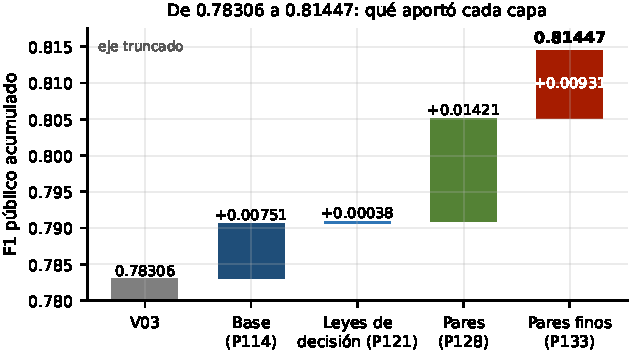
\includegraphics[width=0.92\columnwidth]{fig_waterfall.pdf}
\caption{Descomposición de la ganancia del leaderboard por capas. El eje
está truncado en 0.780 para hacer visibles las diferencias; la altura de cada
barra es la ganancia acumulada, no el valor absoluto.}
\label{fig:waterfall}
\end{figure}

\subsection{El campeón P133}

P133 es un lote de nueve pares: cuatro en HS, dos en TR y tres en AG, con
desplazamientos de $\pm2.05$ en log-odds. Los rescates activan textos con
agresiones severas contra mujeres y xenofobia explícita; las supresiones
desactivan textos de humor de animación y bromas informales que el envío
anterior marcaba como positivos y el leaderboard sugiere que eran falsos
positivos. El envío conserva el
ancla $(514,330,421)$, no presenta violaciones de la regla HatEval y tiene
una huella SHA256
\texttt{b0979a8a\ldots}. En el leaderboard público alcanzó 0.81447, con una
ventaja de $+0.00212$ sobre el segundo clasificado en el momento de la
medición. La Tabla~\ref{tab:serie} y la Figura~\ref{fig:escalera} lo sitúan
como el máximo de la serie en el leaderboard público; su métrica OOF es
idéntica a la de las variantes P127--P133, algo mayor que la de P124--P126
(0.787127) y menor que la de P109.
